\section{Queueing network components}

This chapter presents a comprehensive theoretical analysis of the implemented model.
The following illustration depicts the system components involved in the load test in the context of queuing theory. 

For the purposes of this illustration, let Q\textsubscript{T} represent the thinking station, Q\textsubscript{B} represent the backend, and Q\textsubscript{D} represent the database.

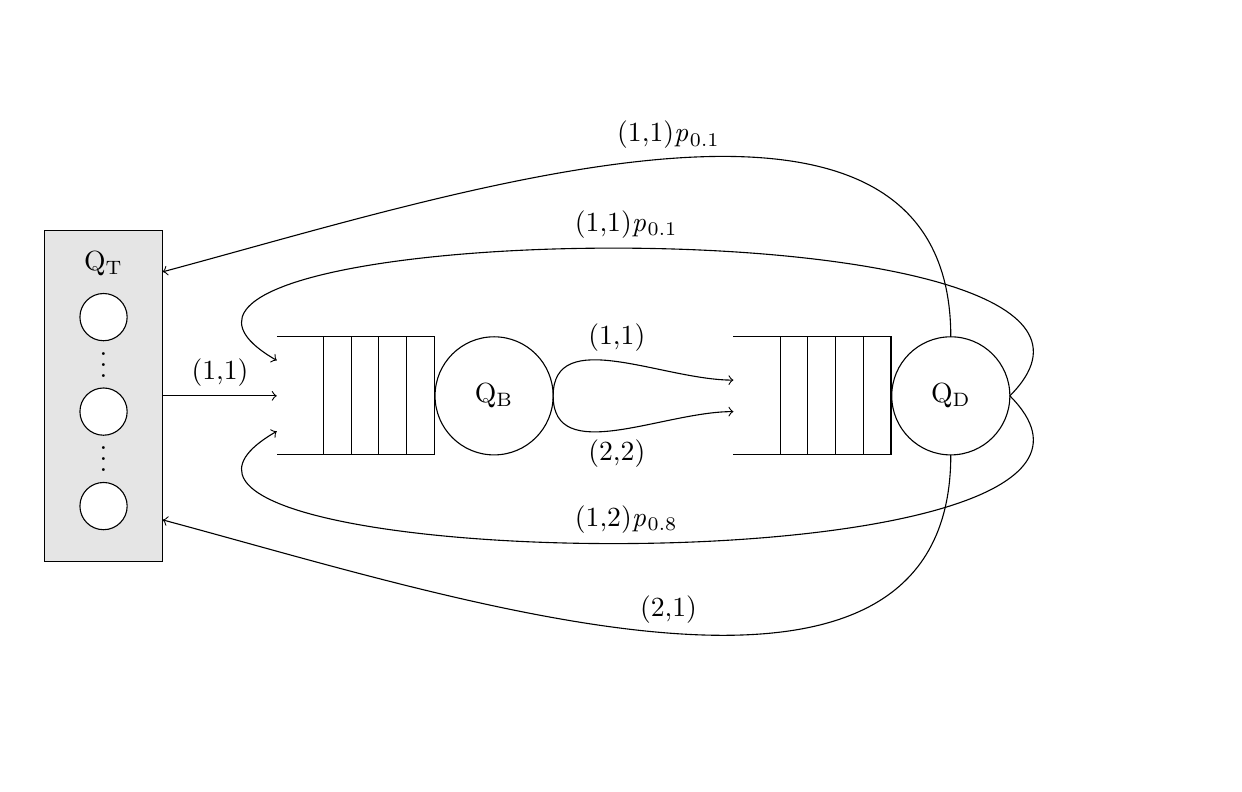
\begin{tikzpicture}
	\tikzstyle{thinking_station} = [rectangle, draw, minimum height=4.2cm, minimum width=1.5cm, fill=gray!20, align=left]
	\tikzstyle{circle_node} = [circle, draw, fill=white, minimum size=6mm, inner sep=0pt]
	\tikzstyle{queue} = [circle, draw, minimum size=1cm, text centered, inner sep=0pt]

	% Thinking station
	\node (QT) [thinking_station] at (0,0) {};
	\node at (0,1.68) {Q\textsubscript{T}};
	% Users belonging to the closed loop
	\node[circle_node] at (0, 1) {};
	\node at (0, 0.5) {$\vdots$};
	\node[circle_node] at (0, -0.2) {};
	\node at (0, -0.7) {$\vdots$};
	\node[circle_node] at (0, -1.4) {};

	% Backend station
	% Queue
	\draw (2.2,0.75) -- ++(2cm,0) -- ++(0,-1.5cm) -- ++(-2cm,0);
	\foreach \i in {1,...,4}
	\draw (4.2cm-\i*10pt,0.75) -- +(0,-1.5cm);
	% Service room
	\draw (4.96,-0.00cm) circle [radius=0.75cm];
	% Label service time
	\node at (4.96,-0.00cm) {Q\textsubscript{B}};

	% Database station
	% Queue
	\draw (8.0,0.75) -- ++(2cm,0) -- ++(0,-1.5cm) -- ++(-2cm,0);
	\foreach \i in {1,...,4}
	\draw (10cm-\i*10pt,0.75) -- +(0,-1.5cm);
	% Service room
	\draw (10.760,-0.00cm) circle [radius=0.75cm];
	% Label service time
	\node at (10.760,-0.00cm) {Q\textsubscript{D}};

	\draw[->]	(QT) to[out=0,in=180] node[above]	{(1,1)} (2.2,0);
	\draw[->]	(5.71,0) to[out=90,in=180] node[above]	{(1,1)} (8.0,0.20);
	\draw[->]	(5.71,0) to[out=-90,in=180] node[below]	{(2,2)} (8.0,-0.20);
	\draw[->]	(11.51,0) to[out=45,in=150] node[above]	{(1,1)\textit{p}\textsubscript{0.1}} (2.2,0.45);
	\draw[->]	(11.51,0) to[out=-45,in=-150] node[above]	{(1,2)\textit{p}\textsubscript{0.8}} (2.2,-0.45);
	\draw[->]	(10.760,-0.75) to[out=-90,in=-15] node[above]	{(2,1)} (0.75,-1.575);
	\draw[->]	(10.760,0.75) to[out=90,in=15] node[above]	{(1,1)\textit{p}\textsubscript{0.1}} (0.75,1.575);
\end{tikzpicture}

It is possible to derive several characteristics of the system under consideration from the illustration above.

The system is characterised by a closed and interactive nature, free of stability conditions, and a constant number of users that dictate the nature of the workload.
A further aspect that emerges relates to the multiclass nature of the jobs within the system, as indicated by the labels placed at the station entry and exit arcs.

Subsequently, an in-depth examination will be conducted on the distinct service time/demand and probabilistic routing for the two classes of jobs.

In conclusion, the network under analysis can be classified as a BCMP, exhibiting a closed topology and utilising ``Processor Sharing'' (PS) as its scheduling discipline.

Prior to examining the nature of the queues that characterise our network and their associated scheduling disciplines, we proceed with the formalisation and resolution of the network's traffic equations.
These equations will then be essential in producing the theoretical analysis of the system.

\section{Traffic equations}

The system's traffic equations are presented below.

\[
\begin{cases}
\begin{aligned}
e_{B1} &= e_{T1} + (0.1 \times e_{D1}) \\
e_{B2} &= 0.8 \times e_{D1} \\
e_{D1} &= e_{B1} \\
e_{D2} &= e_{B2} \\
e_{T1} &= e_{D2} + (0.1 \times e_{D1}) \\
\end{aligned}
\end{cases}
\Rightarrow
\begin{cases}
\begin{aligned}
% Insert your new system here, for example:
e_{B1} &= \num[round-mode=places, round-precision=4]{1.11111111111111} \times e_{T1}  \\
e_{B2} &= \num[round-mode=places, round-precision=4]{0.888888888888889} \times e_{T1}  \\
e_{D1} &= \num[round-mode=places, round-precision=4]{1.11111111111111} \times e_{T1}  \\
e_{D2} &= \num[round-mode=places, round-precision=4]{0.888888888888889} \times e_{T1}  \\
\end{aligned}
\end{cases}
\]

The system of equations above demonstrates that our routing is irreducible, which implies that any queue can be accessed from any other queue within the network.
From an analytical standpoint, our system is under-determined, indicating the existence of an infinite number of solutions. The non-trivial solutions can be derived from the non-zero multiplicative coefficients.

Moreover, it is essential to highlight that within this context, where the system under consideration is an interactive queueing network, it is imperative to impose an additional constraint on the previous system, specifically $e_{T1}=1$, given that this is the thinking station Q\textsubscript{T}.

\section{Queueing systems analysis}

This section will provide a brief overview of the components of our network, with reference to Kendall's notation.

\subsection{Thinking station}

The thinking station can be represented by a queuing system described with the \newline ``G/D/$\infty$/IS'' notation.
The distribution of inter-arrival times for jobs at the thinking station is unknown, but the distribution of service times is known, as the jobs within it remain in service (\textit{thinking state}) for a fixed constant time, known as thinking time.
By definition, the thinking station is equipped with an infinite number of servers, indeed an undefined number of jobs can access it.
Consequently, the service discipline of this system is of the ``Delay center'' or ``Infinite Servers'' type, as all the jobs remain in an idle state in parallel.

\subsection{Backend station}

With regard to the JavaScript runtime environment Node.js, despite its reputation as a ``purely single-threaded'' execution environment due to its Event Loop, it is in fact capable of offloading I/O blocking operations to separate threads or the operating system, thus allowing the main thread to continue processing other tasks.
The library that permits the dispatching of blocking operations to a thread pool is called \verb|libuv| and it belongs to the Chrome V8 Engine.
Furthermore, Node.js has also implemented the \verb|worker_threads| module, which allows for further enhancements of performance by the utilisation of multi-core processors for CPU-bound operations.

In light of the aforementioned considerations, it can be concluded that the RESTful API functions as a ``G/G/1/PS'' queueing system.
This is due to the fact that no manual instantiation of multiple worker threads was performed for the API, and thus a unique main thread is responsible for handling all incoming requests through a ``Processor Sharing'' scheduling discipline.

\subsection{Database station}

With regard to MongoDB, an examination of the ``Production Notes'' section reveals that its WiredTiger storage engine is inherently multithreaded.
In particular, the total number of active threads (i.e. concurrent operations) relative to the number of available CPUs can impact performance as follows:

\begin{itemize}
	\item The throughput increases in direct proportion to the number of concurrent active operations, up to the overall number of CPUs.
	\item The throughput decreases as the number of concurrent active operations exceeds the number of CPUs by a certain threshold amount.
\end{itemize}

The optimal number of concurrent active operations for a given application can be determined through the measurement of throughput.

In order to ascertain the exactness of the information provided in the documentation, an empirical test was conducted to monitor the thread pool instantiated by the MongoDB service in both idle and stressed states.

The results obtained from the Linux command-line utility \verb|htop| are presented below.

\begin{figure}[h]
    \centering
    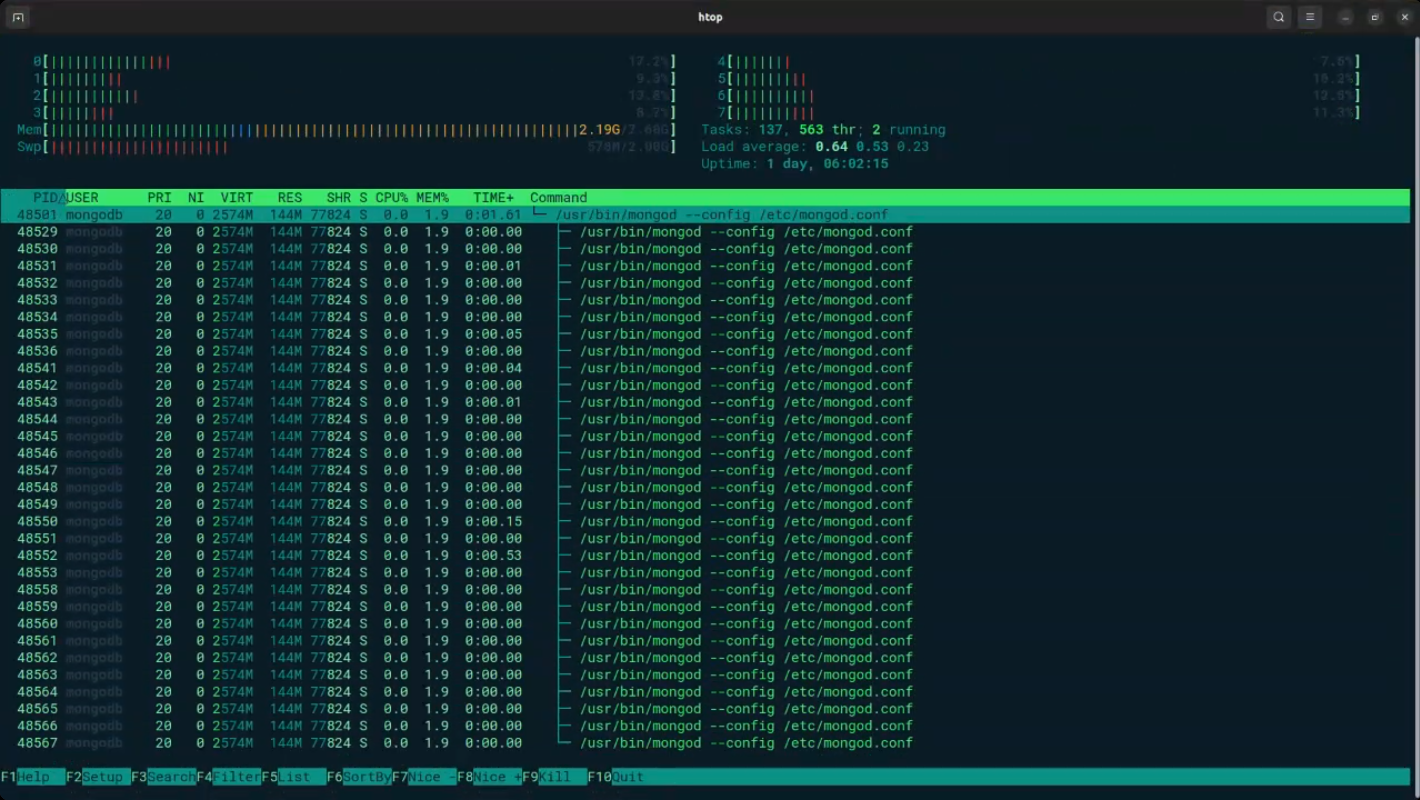
\includegraphics[width=\linewidth]{mongo-idle.png}
    \caption{MongoDB thread pool in idle state}
\end{figure}

\begin{figure}[h]
	\centering
	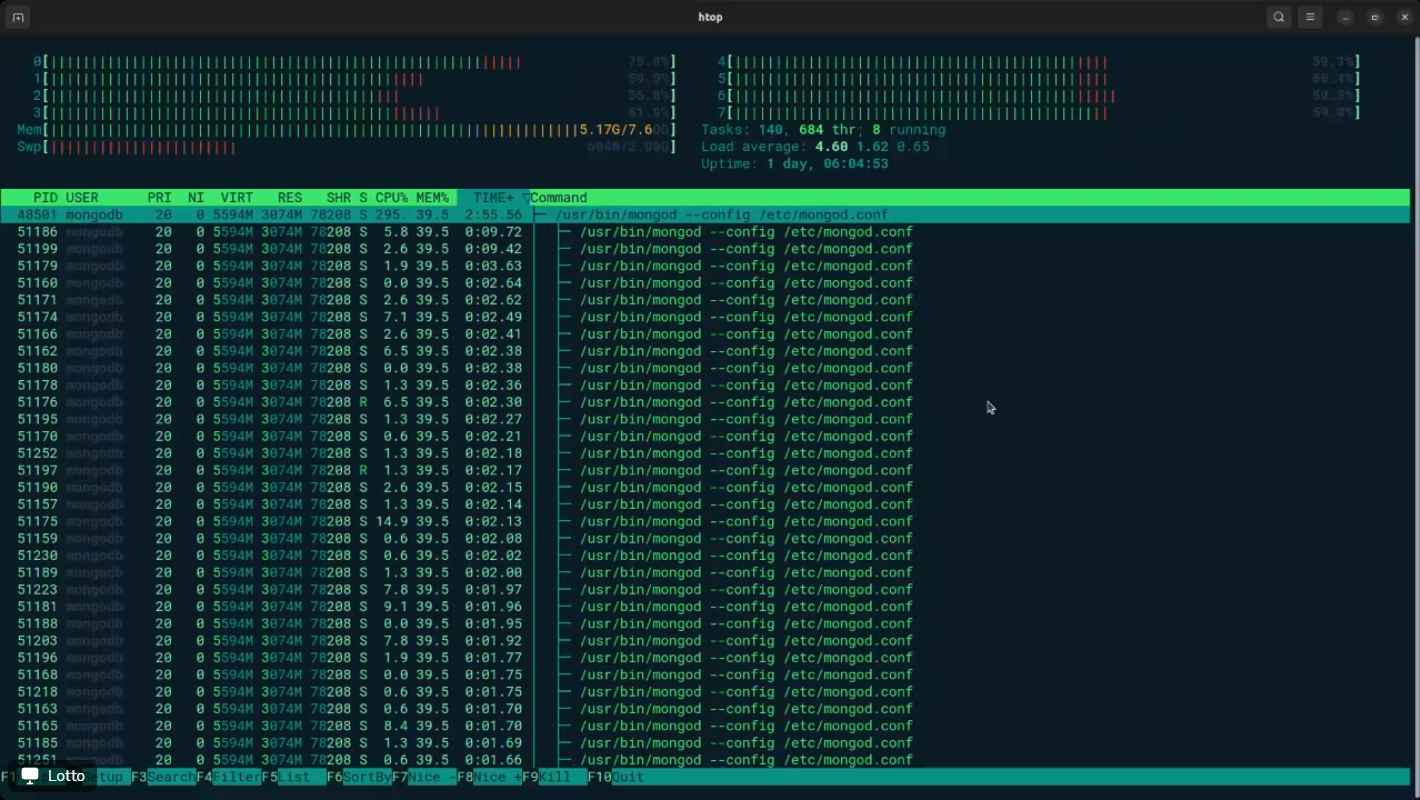
\includegraphics[width=\linewidth]{mongo-stress.png}
	\caption{MongoDB thread pool under load conditions}
\end{figure}	

In conclusion, the database can be identified as a ``G/G/\#C/PS'' queueing system, where ``\#C'' represents the number of cores.
The inter-arrival times and service times are both unknown, however it can be stated that the database leverages all CPU cores with a ``Processor Sharing'' service discipline.
